\chapter{Data Processing and Feature Construction}
\label{chap:data-processing-and-feature-construction}

The WeiMai social marketing context, raw data sources, staged cleaning scope, three units of analysis, main outcome variables, and principal data limitations define what the data are. The data-processing workflow explains how content features, diffusion measures, and content–agent matching variables were constructed, and how each variable's modelling role was fixed before estimation.

\section{Overview of the Data-Processing Pipeline}
\label{sec:4-1-overview-of-the-data-processing-pipeline}

The empirical analysis is built on a staged data-processing pipeline that moves from raw behavioural and article data to level-specific empirical datasets. Figure 4.1 summarises the four stages: WeChat data preparation, LLM-assisted content feature construction, diffusion-network reconstruction, and final dataset and matching-variable assembly. This staged structure makes the workflow auditable, allows individual stages to be re-run without rebuilding the entire dataset, and records the provenance of each analytical variable.

\begin{figure}[H]
\centering
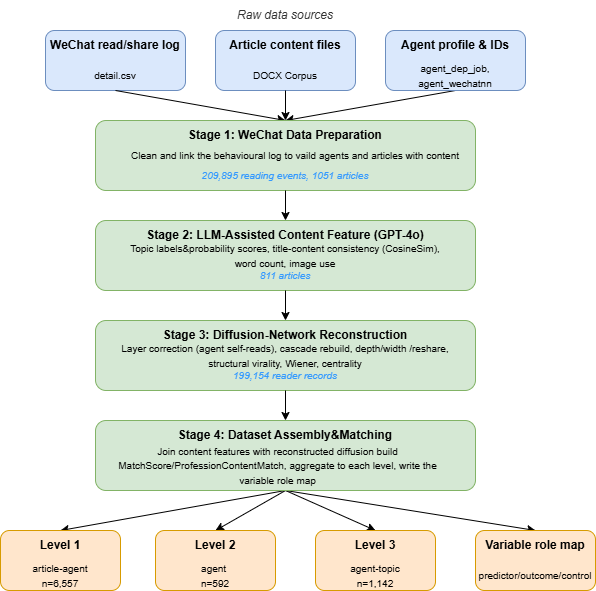
\includegraphics[width=0.92\textwidth]{figures/figure_4_1_workflow.png}
\caption{Overall data-processing workflow from raw sources to the three-level empirical datasets.}
\label{fig:4-1}
\end{figure}

The workflow also produces a variable role map, which classifies variables as outcomes, predictors, controls, or validation-only fields according to whether they exist before diffusion or are reconstructed from realised cascades.

\section{Stage 1: WeChat Data Preparation}
\label{sec:4-2-stage-1-wechat-data-preparation}

Stage 1 prepared an event-level behavioural dataset that is internally consistent and that can be linked across the three raw data sources: the WeChat reading and sharing log, the article documents, and the agent organisational profile and identifier records. At this stage the objective was not to construct the final modelling variables, which are derived in Stages 2 to 4, but to form a clean, linkage-consistent, event-level behavioural foundation on which those later variables could be built. Concretely, this meant ensuring that every reading record retained for later analysis could be connected to a valid agent and to an article whose content could subsequently be processed.

The agent records were prepared first. The organisational profile table was filtered to retain only agents whose department and job fields were both present and non-empty. The agent identifier (\varname{agent\_name}) was normalised by trimming surrounding whitespace and treating empty strings as missing, and the corresponding key column in the profile table was renamed to a common name, so that agents could be matched consistently across the three sources. The filtered profile table was then combined with the WeChat identifier records through an inner join, so that only agents with both complete organisational attributes and a usable WeChat identifier were carried forward. Agents that could not be linked on both sides could not support the later agent-characteristic and content–agent matching analyses.

The behavioural log was then cleaned and restricted in two steps. First, records with \varname{reader\_gender} == 2, treated in the processing notebook as an undefined or unusable gender code, were removed to ensure later gender-composition and assortativity measures were not biased by unusable codes. Second, the log was restricted to readings associated with the linked agents prepared above. After this initial reader-and-agent linkage filtering, the retained behavioural table contained 258,179 records.

The behavioural records were then restricted to articles whose content could be processed. Because the study examines the relationship between article content and diffusion, a reading record was usable only if its article could be matched to a corresponding document file through the title–path index. After this content-linkage restriction, the main content-linked behavioural table contained 209,895 records across 1,051 articles. This table formed the event-level foundation that was carried forward into Stage 3, where it was used to reconstruct the article–agent diffusion cases that constitute the Level 1 unit of analysis.

\section{Stage 2: LLM-Assisted Content Feature Construction}
\label{sec:4-3-stage-2-llm-assisted-content-feature-construction}

Stage 2 transformed the unstructured article documents into structured content variables. The WeChat behavioural records prepared in Stage 1 identify which articles were shared and read, but they do not directly describe the substantive meaning, topic, length, or visual presentation of each article. Since the dissertation examines whether article content characteristics are associated with diffusion effectiveness, it was necessary to convert the original DOCX article files into measurable content features that could be joined to the behavioural and diffusion datasets.

The article files contained several types of information: the article title, body text, and embedded images. These components are important because marketing articles are not only textual objects. In the interior design and home decoration context, images may communicate design style, product quality, decoration examples, or lifestyle atmosphere. At the same time, the title provides the first cue that readers encounter, while the body text develops the article’s substantive content. Stage 2 processed both textual and visual components.

The first step was document extraction. For each DOCX file, the pipeline extracted the article title, body text, article length, and embedded image information. The extracted title was used to represent the article’s initial message cue, while the body text represented the fuller substantive content. Article length was stored as \varname{WordCount}. However, because the articles are Chinese-language marketing documents, this variable should be interpreted as an extracted text-length measure, not as a literal English word-count measure. Image information was also retained, including whether the article contained at least one image and the number of extracted images. These variables later entered the empirical analysis as content metadata and controls.

The second step was LLM-assisted topic extraction. For each article, the model generated topic descriptions at two levels. \varname{Title\_Topics} described the themes suggested by the article title, while \varname{Combined\_Topics} described the themes reflected in the title together with the body text and available image context. An article’s title and full content may not always communicate exactly the same theme. The title may emphasise a promotional hook or a broad lifestyle idea, whereas the article body may focus on renovation, design services, real estate, branding, or customer management. Generating both title-level and combined-content topic descriptions made it possible to examine not only what the article was about, but also how consistently the title and content were aligned.

The six topic categories used in the final empirical analysis were not predefined theoretical categories. Instead, they were inductively derived from the article corpus during the Stage 2 LLM-assisted content construction process. After the initial extraction and cleaning steps, the usable content-modelling corpus contained 814 articles. The topic terms generated in \varname{Title\_Topics} and \varname{Combined\_Topics} were then pooled together across these articles. This produced 4,070 topic terms in total, which were reduced to 1,386 unique topic terms after deduplication. The purpose of this step was to identify recurring semantic themes in the corpus instead of imposing topic categories in advance.

The pooled topic list was then submitted to GPT-4o for higher-level semantic consolidation. The model was instructed to group semantically similar topic terms into approximately five to six broader clusters that could represent the major content themes in the article corpus. The actual output contained six Chinese topic clusters: {\cjkfont 家居设计与装修}, {\cjkfont 房地产与建筑}, {\cjkfont 活动与促销}, {\cjkfont 品牌与市场推广}, {\cjkfont 生活方式与文化}, and {\cjkfont 客户服务与管理}. These categories were then translated and standardised into the English canonical labels used in the Stage 4 empirical analysis: Home Design \& Decoration, Real Estate \& Architecture, Events \& Promotions, Brand \& Marketing, Lifestyle \& Culture, and Customer Service \& Management. The full extraction prompt, the clustering parameters, and the complete Chinese--English topic-label mapping are provided in Appendix~\ref{app:content-feature-extraction}.

This process means that the final six-cluster structure should be interpreted as a corpus-derived topic taxonomy. It summarises the dominant themes observed in the WeiMai article collection and is not an externally imposed theoretical classification. The Chinese labels preserve the original topic-clustering output, while the English canonical labels provide a consistent modelling and reporting vocabulary. The use of English labels in the final analysis avoids mixing Chinese and English topic names within the same regression tables, figures, and thesis text.

After the six-cluster taxonomy had been defined, each article was represented through topic-probability scores as well as a dominant label. Marketing articles may cover more than one theme. For example, an article may primarily discuss home decoration while also containing promotional or brand-related elements. A hard label would force the article into one category and ignore this mixture. By contrast, topic-probability vectors preserve the distribution of each article across the six clusters. These vectors were produced separately for title-level and content-level representations, allowing the analysis to compare the article’s initial framing with its fuller substantive meaning.

Two dominant-topic fields were generated from these topic representations. The title-level field, \varname{TopTitleCluster}, identifies the dominant topic in the title-level representation and is mainly used as a descriptive or intermediate field for understanding how an article is initially framed. The content-level field, \varname{TopContentCluster}, identifies the dominant topic in the full content-level representation and serves as the main topic category used in the empirical analysis. Since the body content provides a more complete representation of the article than the title alone, \varname{TopContentCluster} is treated as the primary topic variable in the Level 1 content model and as a topic control in the Level 3 matching model. Topic labels were standardised into the six canonical English categories before the Stage 4 modelling datasets were assembled.

In addition to topic labels, Stage 2 constructed measures of title–content semantic consistency. The logic is that an article’s title and body content may be more or less aligned. If the title signals one topic but the article body mainly discusses another, readers may experience the article as less coherent or less relevant. Conversely, if the title and body content are semantically consistent, the article may provide a clearer message and maintain reader expectations more effectively. To operationalise this idea, the title-level topic vector and content-level topic vector were compared using vector-based distance and similarity measures.

The primary semantic consistency variable is \varname{CosineSim}, which measures the similarity between the title topic vector and the content topic vector. A higher value indicates stronger title–content alignment in the six-dimensional topic space. Two additional distance measures, \varname{EuclideanDist} and \varname{ManhattanDist}, were also computed as alternative representations of title–content difference. Unlike \varname{CosineSim}, which increases with similarity, these distance measures increase as the title and content vectors become more different. Together, these variables allow the analysis to examine whether semantic consistency is associated with diffusion outcomes and to test whether findings are robust to alternative vector-distance definitions.

Several processing safeguards were used to make the LLM-assisted content outputs suitable for empirical analysis. The classification prompt used a low sampling temperature to improve output stability across articles. Partial outputs were saved during batch processing so that failed or interrupted runs would not require the entire corpus to be processed again. After batch processing, intermediate files were merged, duplicate article records were removed, and topic labels were standardised before the content features were joined to the Stage 4 analysis datasets. These safeguards helped convert LLM outputs into reproducible, table-based content variables instead of leaving them as unstructured text responses.

The reduction in article count occurred during Stage 2 content-feature construction, not during Stage 1 behavioural-data preparation or later diffusion reconstruction. Stage 1 identified 1,051 articles that both appeared in the behavioural records and could be linked to DOCX files. The main reduction occurred when the extracted content outputs were cleaned for content modelling: 237 articles lacked sufficient extracted content or topic information, leaving the 814-article corpus used for topic-term pooling and clustering. Three further articles were then removed because \varname{TopContentCluster} was missing or invalid. After these validity checks, the translated clustered content file used in Stage 4 contained 811 unique article titles.

The 811-article final content-feature source therefore reflects Stage 2 content validity. Stage 4 used these valid, standardised content features and expanded the articles into article–agent and agent–topic observations according to the relevant unit of analysis.

Stage 2 produced three broad groups of article-level content variables. The first group contains topic variables, including the six-cluster topic scores, \varname{TopTitleCluster}, and \varname{TopContentCluster}. The second group contains semantic consistency variables, including \varname{CosineSim}, \varname{EuclideanDist}, and \varname{ManhattanDist}. The third group contains article-format variables, including \varname{WordCount}, \varname{HasImage}, and \varname{NumImages}. Table 4.1 summarises the main content variables generated in this stage.

\begin{table}[H]
\centering
\scriptsize
\caption{Main article content variables generated in Stage 2}
\label{tab:4-1}
\renewcommand{\arraystretch}{1.15}
\begin{tabularx}{\textwidth}{>{\raggedright\arraybackslash}p{0.21\textwidth}>{\raggedright\arraybackslash}p{0.22\textwidth}>{\raggedright\arraybackslash}p{0.28\textwidth}>{\raggedright\arraybackslash}p{0.20\textwidth}}
\toprule
\textbf{Variable group} & \textbf{Variables} & \textbf{Description} & \textbf{Role in later analysis} \\
\midrule
Topic-score representation & Six title/content topic scores & Topic probability vectors across six clusters & Content representation; robustness checks \\
Title dominant topic & \varname{TopTitleCluster} & Dominant title-level topic & Descriptive/intermediate field \\
Content dominant topic & \varname{TopContentCluster} & Dominant full-content topic & Main topic predictor/control \\
Semantic consistency & \varname{CosineSim} & Title–content topic-vector similarity & Main consistency predictor \\
Alternative distance measures & \varname{EuclideanDist}, \varname{ManhattanDist} & Title–content topic-vector distance & Robustness checks \\
Textual format & \varname{WordCount} & Extracted article length & Content metadata control \\
Visual format & \varname{HasImage}, \varname{NumImages} & Image presence and count & Content metadata control \\
\bottomrule
\end{tabularx}
\end{table}

The output of Stage 2 was an article-level content feature table. Each row represented one article and contained its topic labels, topic scores, semantic consistency measures, and format-related variables. This output could then be joined to the cleaned behavioural table from Stage 1 by article title or article identifier. In the Level 1 dataset, these features support the content model by explaining variation across article–agent diffusion cases. In the Level 3 dataset, they support the matching model by providing the article-topic information needed to construct and interpret content–agent alignment.

The LLM-generated outputs are interpreted as constructed content features, not as perfect measures of true article meaning. This limitation is important because article-topic classification may contain uncertainty, especially for articles with mixed themes, short or ambiguous text, promotional language, or image-heavy presentation. Nevertheless, the Stage 2 pipeline provides a consistent and scalable way to convert unstructured marketing articles into structured content variables that can be used in the three-level empirical framework. The next stage uses the cleaned behavioural records to reconstruct the realised diffusion cascades and compute multi-dimensional diffusion measures.

\section{Stage 3: Diffusion Network Reconstruction}
\label{sec:4-4-stage-3-diffusion-network-reconstruction}

Stage 3 converted the cleaned event-level reading records into reconstructed diffusion cascades and computed the multi-dimensional diffusion measures used as outcome variables in the empirical analysis. The raw propagation-layer field in the reading log is not directly usable: agents frequently read and reshare their own articles through their personal accounts, which distorts the recorded layer of the cascade. The stage first corrected the propagation layers, then rebuilt each cascade as a graph, and finally derived cascade-level and graph-theoretic measures from the corrected structure.

Layer correction did not rely on the recorded \varname{reader\_layer} alone. Its central step was the identification of agent self-reads. For each agent, a set of personal WeChat accounts was assembled from the agent's identifier record, which holds up to three WeChat names (\varname{wechat\_1}, \varname{wechat\_2}, and \varname{wechat\_3}) representing the multiple personal accounts a single agent may use. Within each article–agent cascade, a reader was treated as an agent self-read whenever its WeChat name matched any one of the agent's up to three accounts. Readers satisfying this condition were mapped onto a single agent root node. The same rule was applied to the parent linkage, so that a parent share matching any of the agent's accounts was likewise mapped to the agent root. With the agent established as the unique root, each cascade was then rebuilt from the observed sharing edges, and the corrected propagation layer of every reader was taken as its shortest-path distance from the agent root, computed by breadth-first traversal. This procedure prevents an agent's own reading or resharing from being mistaken for ordinary audience diffusion, and it produced the corrected reader-level diffusion table that underlies all subsequent measures.

Figure 4.2 provides an illustrative example of how a reconstructed article–agent cascade can be displayed as a rooted network.

\begin{figure}[H]
\centering
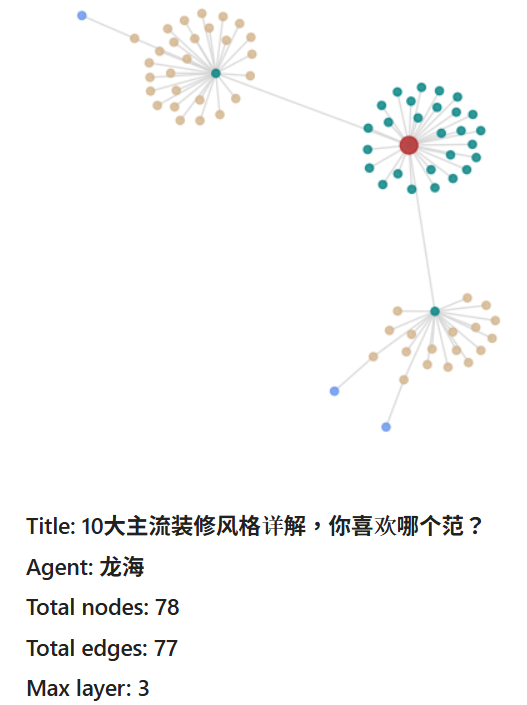
\includegraphics[width=0.58\textwidth]{figures/figure_4_2_cascade_example.png}
\caption{Illustrative reconstructed article–agent diffusion cascade.}
\label{fig:4-2}
\end{figure}

Before metrics were computed, two derived fields were created at the reader level. Dwell time was converted to seconds by multiplying the recorded dwell-time value, which is expressed in fifteen-second units, by fifteen. A reshare flag was set for any reader who shared the article either to their WeChat Moments or directly to friends. Each article–agent pair then defined one cascade, and the cascade-level measures were computed over the readers belonging to that pair. Stage 3 provided the corrected diffusion structure of each cascade. The reach measure used as the primary outcome, \varname{cascade\_size}, and its log transform, \varname{log\_reach} = log(1 + \varname{cascade\_size}), were subsequently derived from this structure in Stage 4, where \varname{cascade\_size} is defined as the total number of reader records in the reconstructed cascade for an article–agent pair.

Several cascade-shape measures were computed from the corrected layers. The first- and second-layer widths count the readers at the first and second propagation layers respectively, and the depth is the maximum corrected layer reached by the cascade. The reshare percentage was computed over the audience only, excluding the agent's own layer-0 record, as the proportion of distinct readers who reshared the article. Reading-duration summaries, including the mean and variance of dwell time, and gender-composition summaries for both the whole cascade and the audience-only subset, were also recorded.

A further set of graph-theoretic measures describes the structural shape of each cascade. From the directed cascade graph, the agent's out-degree centrality and an average out-degree centrality (the directed density of the graph) were computed, together with a graph-level out-degree centralisation index that captures how concentrated the sharing ties are. From the undirected form of the largest connected component, the Wiener index was computed as the sum of the shortest-path distances between all pairs of nodes, and the structural virality was computed as the mean pairwise distance, equal to twice the Wiener index divided by n(n−1) for a component of n nodes. Structural virality distinguishes broadcast-like cascades, in which most adopters are reached directly from the root, from multi-generation cascades that spread through many intermediate sharers \parencite{goel2016}.

A gender-assortativity measure was also computed on the largest connected component to summarise the tendency of ties to connect readers of the same gender. The measure uses only edges for which both endpoints have a known gender. It compares the observed share of same-gender ties with the share expected if ties formed at random given the realised gender mix. The reported value uses a custom normalisation that maps the comparison to a bounded value and returns zero when a cascade contains no usable gendered edges.

Formally, on the largest connected component, let \(n_{11}\) and \(n_{00}\) be the numbers of ties joining two readers of the same gender (both gender 1 and both gender 0, respectively), and let \(n_{01}\) be the number of mixed-gender ties. The total number of usable gendered ties is
\begin{equation}
m = n_{11} + n_{00} + n_{01}.
\end{equation}
When \(m = 0\), the measure is set to zero. Otherwise, the edge shares, same-gender share, random-mixing expectation, and reported index are defined as follows:
\begin{align}
e_{11} &= \frac{n_{11}}{m}, &
e_{00} &= \frac{n_{00}}{m}, &
e_{01} &= \frac{n_{01}}{m}, \\
p_{\mathrm{same}} &= e_{11} + e_{00}, \\
a_{1} &= e_{11} + 0.5 e_{01}, &
a_{0} &= e_{00} + 0.5 e_{01}, \\
p_{\mathrm{expected}} &= a_{1}^{2} + a_{0}^{2}, \\
\varname{gender\_assortativity}
&= \frac{p_{\mathrm{same}} - p_{\mathrm{expected}}}{(1 - p_{\mathrm{expected}}) + 1}.
\end{align}

The numerator \(p_{\mathrm{same}} - p_{\mathrm{expected}}\) and the \(p_{\mathrm{expected}}\) term match the standard Newman assortativity coefficient for a binary attribute. The additional unit in the denominator is a smoothing term, included in the processing notebook to keep the index bounded and numerically stable across the many small or gender-skewed cascades, for which the standard coefficient's \((1 - p_{\mathrm{expected}})\) denominator can approach zero. The resulting index has the same sign as the standard coefficient but a compressed magnitude (observed range approximately [−0.33, 0.25]). It is interpreted only as a relative, within-study indicator of same-gender tie preference and should not be compared directly with assortativity coefficients reported elsewhere.

\begin{table}[H]
\centering
\scriptsize
\caption{Reconstructed diffusion and network measures constructed in Stage 3}
\label{tab:4-2}
\renewcommand{\arraystretch}{1.15}
\begin{tabularx}{\textwidth}{>{\raggedright\arraybackslash}p{0.30\textwidth}>{\raggedright\arraybackslash}X}
\toprule
\textbf{Measure} & \textbf{Definition / construction} \\
\midrule
\varname{cascade\_size} & Reader records in the reconstructed article–agent cascade; basis for \varname{log\_reach} \\
\varname{first\_layer\_width} / \varname{second\_layer\_width} & Number of readers at the first and second corrected propagation layers \\
\varname{depth} & Maximum corrected propagation layer reached by the cascade \\
\varname{reshare\_pct} & Proportion of distinct audience readers (layer ≥ 1) who reshared the article \\
\varname{duration\_mean\_s} & Mean reader dwell time in seconds \\
\varname{centrality} & Graph-level out-degree centralisation \\
\makecell[l]{\varname{agent\_deg\_centrality} /\\ \varname{avg\_out\_degree\_centrality}} & Agent out-degree centrality and directed graph density \\
\varname{wiener\_index} & Sum of pairwise shortest-path distances on the largest connected component \\
\varname{structural\_virality} & Mean pairwise distance: 2 × Wiener index / [n(n−1)] \parencite{goel2016} \\
\varname{gender\_assortativity} & Custom bounded same-gender tie index on usable gendered ties; set to 0 when no usable ties exist \\
\bottomrule
\end{tabularx}
\end{table}

Stage 3 also attached the agent job category used in the agent and matching analyses. Each agent was assigned to one of five role categories, coded 0 to 4: Unknown, Marketing/Operations, Design, Field Sales, and Online Sales/Customer Service. The agent set is defined by the diffusion data itself: the Level 2 agents are those appearing in the cleaned article–agent cascades, not a subset drawn from any external list. Job category was attached as a lookup and was not used as a filter. It was first merged by agent name from a prepared agent-position classification covering 628 agents. For diffusion agents that were not matched there by name, the category was filled by position, using the category recorded for other agents with the same position. Ten of the 592 agents were filled in this way. One had no recorded position and was coded Unknown. The categories group the underlying job titles as follows in Table 4.3:

\begin{table}[H]
\centering
\small
\caption{Agent job categories used in the agent and matching analyses}
\label{tab:4-3}
\renewcommand{\arraystretch}{1.15}
\begin{tabularx}{\textwidth}{>{\raggedright\arraybackslash}p{0.36\textwidth}>{\raggedright\arraybackslash}p{0.25\textwidth}>{\raggedright\arraybackslash}X}
\toprule
\textbf{Code} & \textbf{Job category} & \textbf{Representative job titles} \\
\midrule
0 & Unknown & Missing or unclassifiable job information \\
1 & Marketing/Operations & General manager, store manager, marketing director, operations director \\
2 & Design & Lead, chief, or senior designer; design-department manager \\
3 & Field Sales & Home-renovation consultant; regional or area manager \\
4 & Online Sales/Customer Service & Online sales, customer service, e-commerce roles \\
\bottomrule
\end{tabularx}
\end{table}

Finally, the reconstructed reader-level measures were aggregated into three diffusion tables corresponding to the three units of analysis: an article–agent table with 6,557 cases, an agent table with 592 agents, and an agent–topic table with 1,142 pairs. The agent and agent–topic tables hold averaged forms of the cascade and network measures, such as the mean cascade size, mean depth, and mean centrality, computed across the cases that belong to each agent or agent–topic combination.

All measures constructed in this stage are reconstructed from the realised diffusion process. They describe what was observed after an article was shared, not conditions that were known beforehand. They are treated as primary or supplementary outcomes in the empirical analysis. This treatment is also why the centrality-class measures are not used at the content level: a centrality value computed for a single article–agent case has no clean content-level interpretation. These measures are retained only at the agent and agent–topic levels, where aggregation gives them a coherent meaning, and the Level 1 content dataset does not include them.

\section{Stage 4 Dataset-Construction Features and Content–Agent Matching}
\label{sec:4-5-stage-4-dataset-construction-features-and-content-agent-matching}

Stage 4 contains both dataset-construction and modelling components. The dataset-construction component assembles the three analysis-ready master datasets and derives the additional variables required for later modelling.

Stage 4 performs level-specific assembly. For the Level 1 article–agent dataset, it joins the reconstructed article–agent diffusion table with the Stage 2 content features and derives additional reach and exposure measures from the corrected reader-level diffusion table, including \varname{cascade\_size}, \varname{unique\_reader\_count}, \varname{total\_reads}, \varname{corrected\_depth}, layer-count variables, and log-transformed outcomes such as \varname{log\_reach}. For the Level 2 agent dataset, it starts from the Stage 3 agent-level diffusion table and augments it with prepared agent attributes, including \varname{JobCategory}, \varname{agent\_gender}, \varname{agent\_job}, \varname{agent\_dep}, \varname{article\_count\_per\_agent}, and \varname{log\_article\_count\_per\_agent}. For the Level 3 agent–topic dataset, it performs the main additional aggregation needed for the matching analysis by grouping article–agent records by \varname{agent\_name} and \varname{TopContentCluster}.

The content–agent matching variables operationalise the fit between an article's topical content and the professional context of the agent who shares it. The underlying logic is that agents are not interchangeable broadcasting channels. Articles about home design, real estate, promotional events, brand communication, lifestyle culture, or customer service may be more relevant to some agents than to others, depending on the agent's job category and professional role.

The source matching variables were constructed at the article–agent level after the article topic scores and the agent \varname{JobCategory} had been attached to the reconstructed diffusion table. The continuous matching variable, \varname{MatchScore}, was computed as a weighted alignment between the article's topic profile and the topics treated as professionally relevant to the agent's job category. For each article–agent case, the article's six-topic probability vector was normalised to sum to one. The job-category relevance vector was normalised so that its largest element equalled one. \varname{MatchScore} was then calculated as the dot product of the two normalised vectors. Higher values indicate stronger alignment between the article's topic mix and the professional role of the sharing agent.

The job-topic relevance weights were manually specified from the functional interpretation of the five job categories above. They were not estimated from diffusion outcomes and were not generated by the LLM content pipeline.

\begin{table}[H]
\centering
\small
\caption{Job categories and topic weights used for content–agent matching}
\label{tab:4-4}
\renewcommand{\arraystretch}{1.15}
\begin{tabularx}{\textwidth}{>{\raggedright\arraybackslash}p{0.30\textwidth}>{\raggedright\arraybackslash}X}
\toprule
Job category & Topic relevance weights \\
\midrule
Unknown & No defined relevance; all weights = 0 \\
Marketing/Operations & Events \& Promotions (1.0), Brand \& Marketing (1.0), Lifestyle \& Culture (1.0) \\
Design & Home Design \& Decoration (1.0), Real Estate \& Architecture (0.5), Lifestyle \& Culture (0.5) \\
Field Sales & Events \& Promotions (1.0), Brand \& Marketing (1.0), Customer Service \& Management (0.5), Home Design \& Decoration (0.25), Lifestyle \& Culture (0.25) \\
Online Sales/Customer Service & Events \& Promotions (1.0), Brand \& Marketing (1.0), Customer Service \& Management (1.0), Home Design \& Decoration (0.25), Lifestyle \& Culture (0.25) \\
\bottomrule
\end{tabularx}
\end{table}

A binary matching indicator, \varname{ProfessionContentMatch}, was then derived by classifying an article–agent case as matched when its \varname{MatchScore} reached or exceeded a threshold of 0.5, and as unmatched otherwise. The continuous and binary measures capture the same underlying construct at different resolutions: \varname{MatchScore} expresses the intensity of content–agent alignment, while \varname{ProfessionContentMatch} expresses whether a case clears a fit threshold. Because \varname{ProfessionContentMatch} is derived from \varname{MatchScore}, the continuous and binary matching measures are not included together in the same regression model.

For the Level 3 dataset, article–agent observations were aggregated to the agent–topic level. Article topic labels were first standardised to the six English canonical categories. The article–agent records were then grouped by \varname{agent\_name} and \varname{TopContentCluster}. Within each agent–topic cell, \varname{MatchScore} was averaged to form \varname{MatchScore\_mean}, and the median value was retained as \varname{MatchScore\_median}. \varname{ProfessionContentMatch\_mean} was calculated as the mean of the binary matching indicator and should be interpreted as a proportion: it measures the share of article–agent cases within the cell that were classified as professionally matched.

This aggregation changes the interpretation of the matching variables. At the article–agent level, \varname{MatchScore} describes the fit between one article and one agent. At the agent–topic level, \varname{MatchScore\_mean} describes the average fit between an agent and a content category across all observed article–agent cases in that cell. Similarly, \varname{ProfessionContentMatch\_mean} is not a binary variable at Level 3. A value close to one indicates that most observed cases in the agent–topic cell were professionally matched, while a value close to zero indicates weak or infrequent matching.

During the same Stage 4 aggregation process, several additional Level 3 controls were constructed. \varname{agent\_topic\_article\_n} counts the number of article–agent cases in each agent–topic cell, and \varname{log\_agent\_topic\_article\_n} is its log-transformed version. These variables control for the amount of observed content evidence available for each agent–topic combination. The pipeline also created sparse-cell indicators, \varname{is\_sparse\_cell\_10} and \varname{is\_sparse\_cell\_30}, to flag cells with fewer than 10 or fewer than 30 observed article–agent cases. Aggregated content metadata were retained at the same level, including \varname{WordCount\_mean}, \varname{HasImage\_share}, \varname{NumImages\_mean}, and \varname{CosineSim\_mean}.

\begin{table}[H]
\centering
\scriptsize
\caption{Main Level 3 matching and aggregation variables}
\label{tab:4-5}
\renewcommand{\arraystretch}{1.15}
\begin{tabularx}{\textwidth}{>{\raggedright\arraybackslash}p{0.21\textwidth}>{\raggedright\arraybackslash}p{0.22\textwidth}>{\raggedright\arraybackslash}p{0.28\textwidth}>{\raggedright\arraybackslash}p{0.20\textwidth}}
\toprule
Variable & Level & Description & Analytical role \\
\midrule
\varname{MatchScore} & Article–agent source field & Continuous article–agent fit score & Source for Level 3 aggregation \\
\makecell[l]{\varname{ProfessionContent}\\\varname{Match}} & Article–agent source field & Binary professional match indicator & Source for Level 3 aggregation \\
\varname{MatchScore\_mean} & Agent–topic & Average \varname{MatchScore} within an agent–topic cell & Main continuous matching predictor \\
\varname{MatchScore\_median} & Agent–topic & Median \varname{MatchScore} within an agent–topic cell & Supplementary matching descriptor \\
\makecell[l]{\varname{ProfessionContent}\\\varname{Match\_mean}} & Agent–topic & Share of matched cases in the cell & Alternative matching predictor \\
\varname{matched\_case\_count} & Agent–topic & Matched article–agent case count & Descriptive matching count \\
\varname{agent\_topic\_article\_n} & Agent–topic & Article–agent cases in the cell & Exposure/cell-size control \\
\makecell[l]{\varname{log\_agent\_topic}\\\varname{\_article\_n}} & Agent–topic & Log-transformed cell count & Main exposure control \\
\varname{WordCount\_mean} & Agent–topic & Mean article length within the cell & Aggregated content control \\
\varname{HasImage\_share} & Agent–topic & Share of articles with images within the cell & Aggregated content control \\
\varname{NumImages\_mean} & Agent–topic & Mean number of images within the cell & Aggregated content control \\
\varname{CosineSim\_mean} & Agent–topic & Mean title–content consistency & Aggregated content control \\
\varname{is\_sparse\_cell\_10} / \varname{is\_sparse\_cell\_30} & Agent–topic & Cells below 10 or 30 cases & Diagnostic/sensitivity fields \\
\bottomrule
\end{tabularx}
\end{table}

\section{Variable Role Map}
\label{sec:4-6-variable-role-map}

The data-processing workflow also defines a variable role map before estimation. Its purpose is to prevent variables from being used in a way that conflicts with their construction logic, especially where a variable is reconstructed from the realised diffusion process and should not be treated as an ordinary pre-diffusion predictor.

The variable role map was implemented as a structured table in the Stage 4 pipeline. For each variable, the map records the empirical level, source file, modelling role, whether the variable is allowed as a predictor, whether it is allowed as an outcome, and a short interpretation or leakage note. The implementation explicitly defines these columns as variable, level, \varname{source\_file}, role, \varname{allowed\_as\_predictor}, \varname{allowed\_as\_outcome}, \varname{leakage\_note}, and \varname{thesis\_interpretation\_note}. This structure makes the modelling permissions transparent and reproducible.

\begin{table}[H]
\centering
\scriptsize
\caption{Variable roles and modelling permissions across the three empirical levels}
\label{tab:4-6}
\renewcommand{\arraystretch}{1.15}
\begin{tabularx}{\textwidth}{>{\raggedright\arraybackslash}p{0.18\textwidth}>{\raggedright\arraybackslash}p{0.18\textwidth}>{\raggedright\arraybackslash}p{0.18\textwidth}>{\raggedright\arraybackslash}p{0.18\textwidth}>{\raggedright\arraybackslash}p{0.18\textwidth}}
\toprule
\textbf{Level} & \textbf{Main predictors / controls} & \textbf{Primary outcome} & \textbf{Supplementary outcomes} & \textbf{Main restrictions} \\
\midrule
Level 1: Content model & Topic, semantic consistency, and article-format variables & \varname{log\_reach} & Reach/width, depth/reshare, duration, and cascade-structure measures & Excludes agent and matching variables; reconstructed measures remain outcomes \\
Level 2: Agent-characteristic model & Role, gender, and activity controls & Agent mean log reach & Cascade, reshare, depth, structure, centrality, exposure, assortativity, and duration & No matching aggregates \\
Level 3: Content–agent matching model & Fit, topic, role, exposure, and content controls & Agent–topic mean log reach & Cascade, depth, reshare, structure, centrality, and duration & \varname{MatchScore} and binary match estimated separately \\
\bottomrule
\end{tabularx}
\end{table}

This role classification clarifies the difference between predictors, controls, and validation-only fields. Predictors are variables used to test the substantive research questions, such as content characteristics in Level 1, agent attributes in Level 2, and matching variables in Level 3. \varname{Controls} are included to adjust for exposure or content metadata, such as article count, agent–topic article count, image use, or article length. Validation-only fields, such as source labels, join keys, and provenance fields, are retained for checking data quality but are not interpreted as substantive modelling variables.

The variable role map bridges feature construction and model design. It distinguishes how variables are constructed from how they may be used. This distinction is central to the dissertation’s empirical strategy: content, agent, and matching variables are used as explanatory variables only at the level where their interpretation is coherent, while reconstructed cascade and diffusion-network measures are treated as observed diffusion outcomes or supplementary descriptors.
